다음 그림에서 점 $\mathrm{I}$는 $\triangle\mathrm{ABC}$의 내심이고, $\overline{\mathrm{BI}}$의 연장선과 $\overline{\mathrm{AC}}$의 교점을 $\mathrm{D}$, $\overline{\mathrm{CI}}$의 연장선과 $\overline{\mathrm{AB}}$의 교점을 $\mathrm{E}$라 하자. $\angle\mathrm{A} = 50^\circ$ 일 때, $\angle x + \angle y$의 크기는 몇 도인지 구하여라.

\begin{figure}[h]
\centering
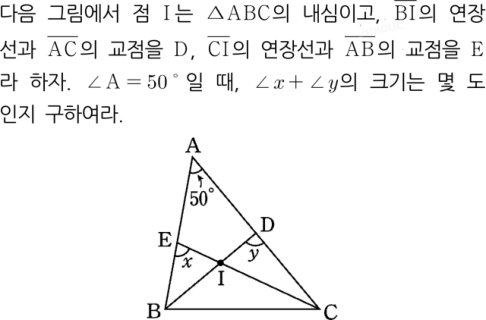
\includegraphics[width=0.3\textwidth]{plain0_problem_09_figure.png}
\end{figure}
